\section{Алгоритмы решения граничных обратных задач. Примеры.}\label{sec:ch4/sec3}

%dvmg368
\subsection{Решение граничной обратной задачи}\label{subsec:ch4/sec3/subsec1}
Пусть функционал $J(\theta)$ удовлетворяет условиям,
указанным в \autoref{subsec:ch2/sec1/subsec3}.
Для удобства введём переобозначение
$\hat{J}(u)\coloneqq J(\theta(u)), \hat{J}:L^2(\Gamma_1) \to \mathbb{R}$.

Здесь $\theta(u)$ -- температурное поле
задачи~\eqref{eq:2_1:initial}--\eqref{eq:2_1:initial-boundary}
отвечающее управлению $u \in L^2(\Gamma_1)$.

Согласно формуле~\eqref{eq:2_1:therorem_2_eq3}
градиент функционала $\hat{J}(u)$~\cite{Grenkin2016a} имеет вид
\[
    \hat{J}'(u)= (\varphi(u) -\theta_b^4)p_2,
\]

где $\varphi(u)$ есть интенсивность излучения,
$p_2$ -- соответствующая переменная сопряжённой системы.

Предлагаемый алгоритм решения выглядит следующим образом:

%\begin{algorithm}[H]
%    \caption{Алгоритм градиентного спуска с проекцией}
%    \begin{algorithmic}[1]
%        \State Выбираем значение градиентного шага $\lambda$,
%        \State Выбираем количество итераций $N$,
%        \State Выбираем произвольное $u_0 \in U_{ad}$,
%        \For{$k \gets 0,1,2,...,N$}
%            :
%            \State Для полученного $u_k$ расчитываем состояние $y_k = \{\theta_k, \varphi_k\}$ из  (\ref{weak_operational}).
%            \State Расчитываем значение функционала качества $J(\theta_k)$ из (\ref{quality}).
%            \State Расчитываем сопряжённое состояние $p_k=\{p_{1k},p_{2k}\}$ из уравнений \eqref{eq:2_1:therorem_2_eq1}--\eqref{eq:2_1:therorem_2_eq2}, где $ \hat{\theta} := \theta_k, \hat{u}=u_k$.
%            \State Пересчитываем управление $u_{k+1} = P_{ad}\left[ u_k - \lambda (\varphi_k - \theta_b^4)p_{2k} \right]$.
%        \EndFor
%    \end{algorithmic}
%\end{algorithm}

\textbf{Algorithm: Gradient Descent with Projection}

1.\ Choose the gradient step value $\lambda$.

2.\ Choose the number of iterations $N$.

3.\ Select an arbitrary initial value $u_0 \in U_{ad}$.

4.\ For $k = 0, 1, 2, \dots, N$:

\hspace{1cm} a.\ Calculate the state $y_k = \{\theta_k, \varphi_k\}$
from equation~\eqref{eq:2_1:weakOperational} for the given $u_k$.

\hspace{1cm} b.\ Calculate the quality functional value
$J(\theta_k)$ from equation~\eqref{eq:2_1:quality}.

\hspace{1cm} c.\ Calculate the conjugate state $p_k = \{p_{1k}, p_{2k}\}$
from equations~\eqref{eq:2_1:therorem_2_eq1}--\eqref{eq:2_1:therorem_2_eq2},
where $\hat{\theta} = \theta_k$ and $\hat{u} = u_k$.

\hspace{1cm} d.\ Update the control $u_{(k+1)} = P_{ad} [ u_k -
\lambda(\varphi_k - \theta_b^4) p_{2k} ]$.

\textbf{End of algorithm.}

Оператор проекции $P_{ad} : U \to U_{ad}$ определён следующим образом
\[
    P_{ad}[v] =
    \begin{cases}
        u_1, & \text{если } v \le u_1 \\
        v, & \text{если } u_1 < v < u_2 \\
        u_2, & \text{если } v \ge u_2.
    \end{cases}
\]
Приведём далее примеры расчётов для двумерного случая.
Положим $\Omega = \{(x,y), 0 \leq x,y \leq 1\}$, $l = 1$ см.
Граница $\partial\Omega$ состоит из участков:
\[
    \begin{aligned}
        \Gamma_0 & = \{x=\{0,1\}, y \in [0,1]\} \\
        \Gamma_1 & = \{x\in [0,1], y=0\}
        - \text{участок с неизвестными отражающими свойствами}, \\
        \Gamma_2 & = \{x \in [0,1], y=1\} - \text{участок наблюдения}.
    \end{aligned}
\]
Будем также далее считать, что $a = 0.006[\text{см}^2/\text{c}]$,
$b=0.025[\text{см}/\text{с}]$, $\beta = 0.00005[\text{см}/\text{с}]$,
$\kappa=1[\text{см}^{-1}]$, $\kappa_s = 0$, $A = 0$, $\gamma = 0.3$.
Указанные параметры соответствуют стеклу~\cite{Grenkin2016a}.
Температуру на границе $\Omega$ положим равной $\theta_b = (x^2+y^2)/3$.

При указанных параметрах для первого эксперимента выберем следующее тестовое
значение функции $u$ (рис.~\ref{fig:4_3:control}\subref{fig1:exp1}):
\begin{equation}
    \label{eq:4_3:equation}
    u(x)=
    \begin{cases}
        0.01, & \text{если } x \le 0.5, \\
        0.5, & \text{если } x > 0.5,
    \end{cases}
\end{equation}
и для второго эксперимента (рис.~\ref{fig:4_3:control}\subref{fig1:exp2}):
\begin{equation}
    \label{eq:4_3:test_function_1}
    u(x)=0.49x+0.01.
\end{equation}

Вычислим решение прямой
задачи~\eqref{eq:2_1:initial}--\eqref{eq:2_1:initial-boundary}
для этих случаев.
Полученное температурное поле на участке наблюдения
$\Gamma_2$ выберем в качестве $\theta_0$.
Далее, применяя предложенный алгоритм находим квазирешение обратной
задачи~\eqref{eq:2_1:initial}--\eqref{eq:2_1:theta_gamma}.
Эффективность алгоритма, а также значение $u_0$ в первом и
втором случаях иллюстрируются рис.~\ref{fig:4_3:control}.
На рис.~\ref{fig:4_3:cost} показана динамика функционала качества по итерациям.

\textbf{Замечание.} В предложенных примерах потребовалось
$2*10^6$ итераций для нахождения квазирешения $u$.
В то же время температурное поле на участке наблюдения
$\Gamma_2$ становится близким к $\theta_0$ уже на $10^2$ итерации.
Также наблюдается существенное падение скорости уменьшения функционала
качества с каждой итерацией после того, как среднее значение найденной
функции контроля становится близко к тестовой функции.
\begin{figure}[]
    \centering
    \subfloat[Первый эксперимент]
    {
        \label{fig:4_3:1}
        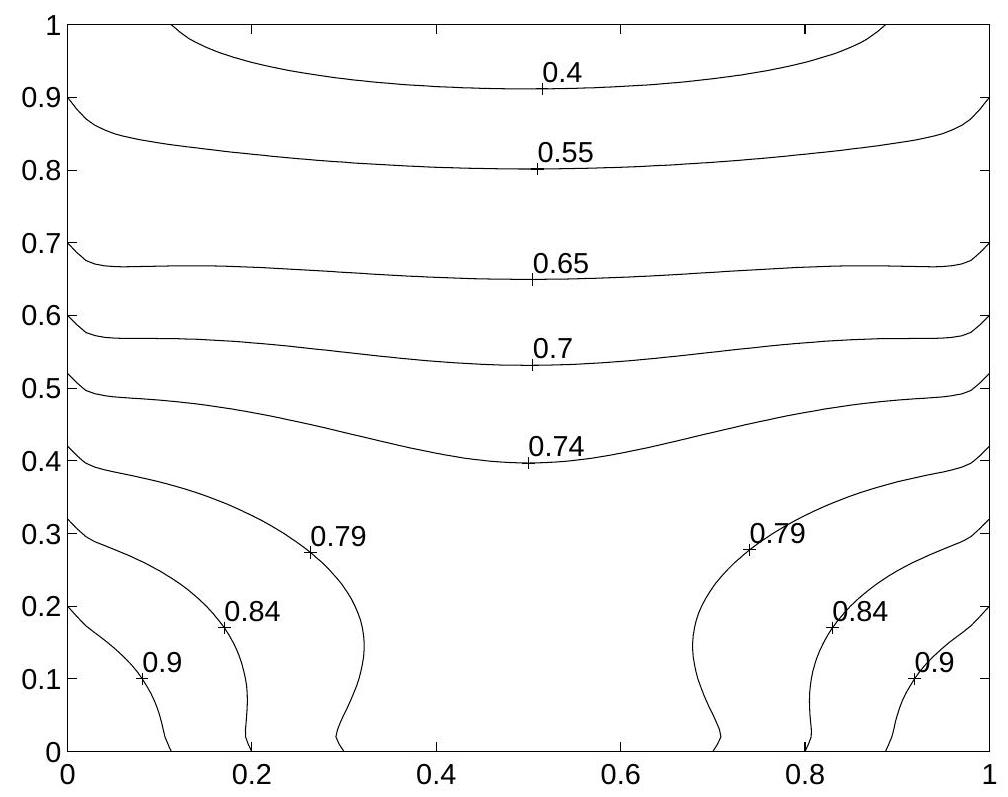
\includegraphics[width=.51\linewidth]{dvmg368/1}
    }
    \subfloat[Второй эксперимент]
    {
        \label{fig:4_3:2}
        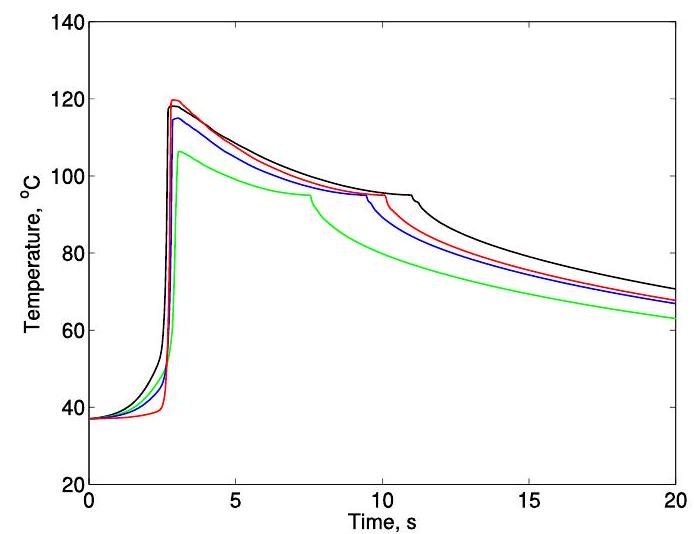
\includegraphics[width=.51\linewidth]{dvmg368/2}
    }
    \caption{Тестовая функция $u$, начальная $u_0$, найденная функция $u_{end}.$}
    \label{fig:4_3:control}
\end{figure}

\begin{figure}[]
    \centering
    \subfloat[Первый эксперимент]
    {
        \label{fig:4_3:exp1}
        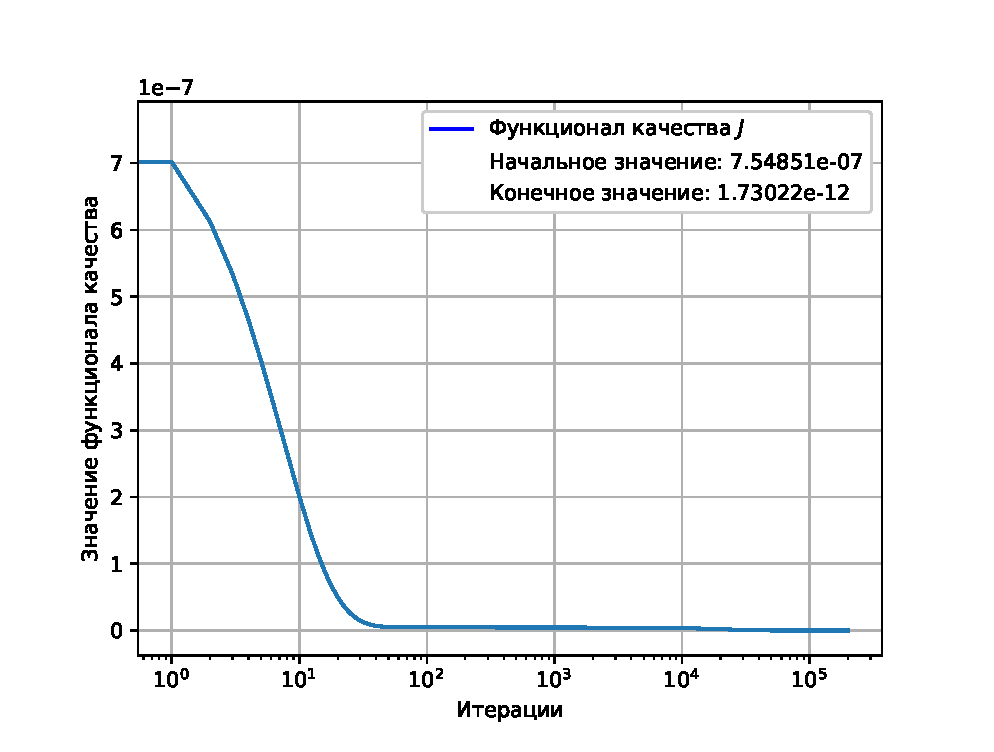
\includegraphics[width=.51\linewidth]{dvmg368/3}
    }
    \subfloat[Второй эксперимент]
    {
        \label{fig:4_3:exp2}
        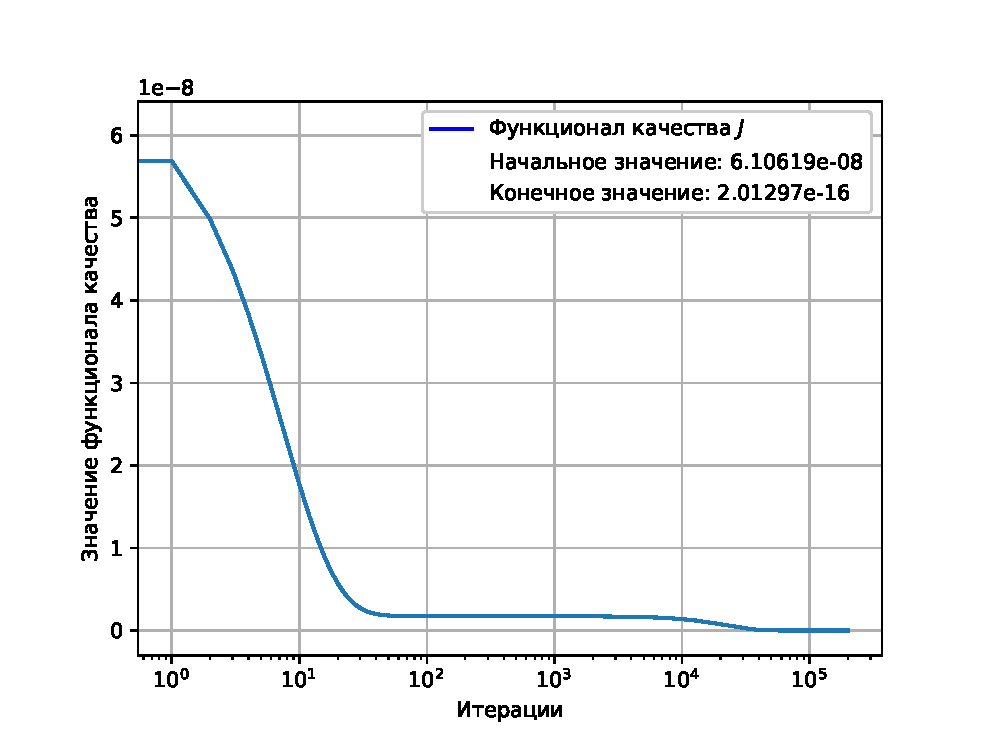
\includegraphics[width=.51\linewidth]{dvmg368/4}
    }
    \caption{Динамика функции $\hat{J}(u)$ по итерациям.}
    \label{fig:4_3:cost}
\end{figure}


%dvmg425
\subsection{Решение краевой задачи
радиационного теплообмена
без условий для интенсивности излучения
}\label{subsec:ch4/sec3/subsec2}

%paper03
\subsection{Решение квазистационарной задачи}\label{subsec:ch4/sec3/subsec3}

%6_Chebotarev
\subsection{Решение квазилинейной модели}\label{subsec:ch4/sec3/subsec4}

%Chebotarev_2 nd, Chebotarev_Park_Mesenev_Kovtanyuk_21
\subsection{Решение задачи с фазовыми ограничениям}\label{subsec:ch4/sec3/subsec5}

